\section{Theorie, nach \cite{Anleitung}}
\label{sec:theorie}
\subsection{Glühelektrischer Effekt}
Beim glühelektrischen Effekt geht es darum, mithilfe von Wärme, Elektronen
aus einem Metall zu lösen. Metalle können häufig als kristalliner Festkörper
beschrieben werden, das bedeutet sie bestehen aus einem Ionengitter. Dabei sind die
Metallionen im inneren praktisch vollständig ionisiert. Das Gitterpotential ist
dadurch weitestgehend konstant und unterscheidet sich vom Außenraum um den Betrag $φ$.
Die Ionen, sogenannte Leitungselektronen, können sich frei bewegen.
Sie sind für die Leitfähigkeit des Metalls verantwortlich.
Die Elektronenemission kann aus quantenmechanischer Betrachtung durch das
Potentialtopfmodell erklärt werden.
\\
Die Elektronen befinden sich in einem Potentialtopf\footnote{Die Skizze wurde mit Tikz erstellt.} der Höhe $ξ$ und müssen die
Austrittsarbeit $\symup{e_0} \: ξ$\footnote{$e_0 = \text{Elementarladung}$}
leisten um den Potentialtopf zu verlassen.

\begin{figure}
      \begin{center}
            \begin{circuitikz}
                  \draw[very thick] (0,0) -- (2,0) -- (2,-2) -- (4,-2) -- (4,0) -- (6,0);
                  \draw (4,-2) (5.2,-2);
                  \draw[<->] (4.8,0) -- (4.8,-2) node[right] at (4.8,-1) {$ξ$};
                  \draw[->] (0,-2.3) -- (2,-2.3) node[below] at (1,-2.3) {$\text{Vakuum}$};
                  \draw[<->] (2,-2.3) -- (4,-2.3) node[below] at (3,-2.3) {$\text{Metall}$};
                  \draw[<-] (4,-2.3) -- (6,-2.3) node[below] at (5,-2.3) {$\text{Vakuum}$};
            \end{circuitikz}
      \end{center}
      \caption{Potentialtopfmodell eines Metalls.}
      \label{fig:pot}
\end{figure}

Die spontane Emission lässt sich mittels der Fermi-Dirac'schen
Verteilungsfunktion darstellen.
\begin{equation}
  f(\symup{E}) = \frac{1}{\exp \left(\frac{\symup{E}\:-\:ζ}{\symup{kT}}\right)\:+\:1}
\end{equation}

\begin{figure}
  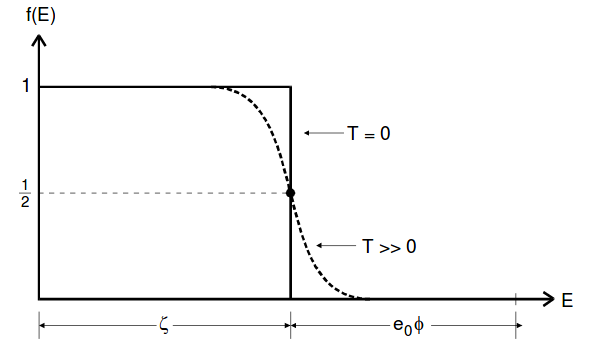
\includegraphics[width=\textwidth]{content/Fermi-Dirac2.png}
  \caption{Fermi-Dirac'sche Verteilungsfunktion\cite{Anleitung}.}
  \label{fig:fermidirac}
\end{figure}

Sie gibt an, mit welcher Wahrscheinlichkeit ein Zustand, im thermischen
Gleichgewicht, die Energie $\symup{E}$ annimmt.

\subsection{Sättigungsstrom}
Um den Sättigungsstrom zu berechnen, also den Strom, welcher pro Zeit -und
Flächeneinheit aus dem Metall fließt, wird die Richardson-Gleichung verwendet.
Sie stellt diesen Zusammenhang in Abhängigkeit von der Temperatur dar
\begin{equation}
  j_\text{S}(\symup{T}) = 4\symup{\pi}\frac{e_0 m_0 \symup{k}^2}{\symup{h}^3}
                      \symup{T}^2 \exp \left(-\frac{e_0 φ}{\symup{kT}}\right)\:.
                      \label{eqn:richardson}
\end{equation}

Um den Sättigungsstrom fehlerfrei messen zu können, müssen die aus der
Metalloberfläche herausgelösten Elektronen abgesaugt werden, damit sie nicht
mit dem Gas wechselwirken. Dies wird zusätzlich durch ein elektrischen Feld
ermöglicht. Eine solche Apparatur wird Hochvakuumdiode genannt und sie wird als
Gleichrichter verwendet.
Hochvakuumdioden können Temperaturen von bis zu $\SI{3000}{\kelvin}$ erreichen.

\subsection{Raumladungsgleichung}
Da die Elektronen wegen der Kathodenspannung eine beschleunigte Bewegung
ausführen, hängt die Raumladungsdichte vom Ort ab. Bei gegebener
Kontinuitätsbedingung der Stromdichte
\begin{equation}
  j = -\symup{ρv}\:,
\end{equation}
gilt also: Die Raumladungsdichte beeinflusst die Feldstärke zwischen Anode und
Kathode.
Als Ansatz wird die Poisson-Gleichung
\begin{equation}
  \increment{\symup{V}} = -\frac{1}{ε_0}ρ
\end{equation}
verwendet. Einfache Umformungen führen auf das Langmuir-Schottkysche
Raumladungsgesetz der Form
\begin{equation}
  j = \frac{4}{9} ε_0 \sqrt{2 \frac{ε_0}{m_0}}\:
      \frac{\symup{V}^\frac{3}{2}}{\symup{a}^2}\:.
  \label{eqn:langmuir}
\end{equation}
Es zeigt den Zusammenhang zwischen der Stromdichte und der Anodenspannung.

\subsection{Kennlinie der Hochvakuumdiode}
Die Kennlinie einer Hochvakuumdiode besteht aus drei Abschnitten. Dem
Anlaufstromgebiet, dem Raumladungsgebiet und dem Sättigungsstromgebiet.
Die Kennlinie wird dazu verwendet um zum einen die Austrittsarbeit der Kathode
und zum anderen die Kathodentemperatur zu bestimmen.

\subsection{Anlaufstrom}
Der Anodenstrom ungleich Null bei $V = 0$ kommt dadurch zustande, dass
die Elektronen eine Eigengeschwindigkeit besitzen. Sie besitzen den
Energieüberschuss
\begin{equation}
  \increment{\symup{E}} = \symup{E} \:-\: \left( ξ \: + \: \symup{e}_0
  \symup{φ} \right)
\end{equation}
welcher als kinetische Energie verstanden werden kann. Dadurch können sie gegen
ein Gegenfeld ankommen. Dieser Strom wird folglich als Anlaufstrom bezeichnet.

\subsection{Kathodentemperatur}
Um die Kathodentemperatur zu berechnen, wird die Leistungsbilanz des
Heizstromfadens herangezogen.
Die zugeführte Leistung beträgt
\begin{equation}
  \symup{N}_\text{zu} = \symup{V}_\text{A} \cdot \symup{I}_\text{A}\:.
\end{equation}
Die Zugeführte Leistung wird in Strahlungsleistung und Wärmeleitung abgegeben.
Dabei kann die Wärmeleitung aus
\begin{equation}
  \symup{N}_\text{WL} = A\:η\:σ\: \symup{T}^4
\end{equation}
berechnet werden.
\\
Nun kann aus
\begin{equation}
  \symup{V}_\text{A} \cdot \symup{I}_\text{A} = A\:η\:σ\: \symup{T}^4 \:
                                          + \: \symup{N}_\text{WL}
                                          \label{eqn:temp}
\end{equation}
die Temperatur der Kathode berechnet werden.
